\documentclass{article}

\usepackage{geometry}
\geometry{
	a4paper,
	total={170mm,257mm},
	left=20mm,
	top=20mm,
}
\usepackage[utf8]{inputenc} % allow utf-8 input
\usepackage[T1]{fontenc}    % use 8-bit T1 fonts
\usepackage[hidelinks]{hyperref}       % hyperlinks
\usepackage{url}            % simple URL typesetting
\usepackage{tikz}
\usepackage{dsfont}
\usepackage{amsmath}
\usepackage{array}
\usepackage{authblk}
\usepackage{float}
\usepackage{rotating}
\usepackage[symbol]{footmisc}
\renewcommand{\thefootnote}{\fnsymbol{footnote}}
\usepackage{makecell}
\usepackage{ragged2e}
\usepackage{array}
\usepackage{longtable}

\usepackage{multirow, makecell}
\renewcommand{\arraystretch}{1.7}
\setlength{\tabcolsep}{12pt}

\graphicspath{{../../figures/}}

\renewcommand{\thefigure}{S\arabic{figure}}
\renewcommand{\thetable}{S\arabic{table}}


\title{Supplementary appendix to: \\ {\Large Historically high excess mortality during the COVID-19 pandemic in Switzerland, Sweden and Spain}}


\author[a,$\dagger$,*]{Kaspar Staub}
\author[b,$\dagger$]{Radoslaw Panczak}
\author[a]{Katarina L. Matthes}
\author[a,c]{Joël Floris}
\author[b]{Claudia Berlin}
\author[d]{Christoph Junker}
\author[d]{Rolf Weitkunat}
\author[e]{Svenn-Erik Mamelund}
\author[b,$\ddagger$]{Marcel Zwahlen}
\author[b,$\ddagger$]{Julien Riou}

\affil[a]{{\small Institute of Evolutionary Medicine, University of Zurich, Switzerland}}
\affil[b]{{\small Institute of Social and Preventive Medicine, University of Bern, Switzerland}}
\affil[c]{{\small Department of History, University of Zurich, Switzerland}}
\affil[d]{{\small Federal Statistical Office, Neuchâtel, Switzerland}}
\affil[e]{{\small Centre for Research on Pandemics \& Society, Oslo Metropolitan University, Norway}}

\affil[$\dagger$] {{\small contributed equally}}
\affil[$\ddagger$] {{\small contributed equally}}
\affil[*] {{\small Corresponding  author (\texttt{kaspar.staub@iem.uzh.ch})}}


\begin{document}
	
	\maketitle
	
	\vspace{-3em}
	
	\tableofcontents
	\clearpage
	
	\section{Material and methods}
	
	The data and the statistical code are available at \url{https://github.com/RPanczak/ISPM_excess-mortality/}.
	
	\subsection{Statistical model}
	
	We built a model where the linear predictor of deaths count in year $i$, month $j$ and age group $k$ $D_{i,j,k}$ depended on (1) an intercept by age group $\alpha_k$, (2) a yearly linear trend $\beta_1$, (3) a periodic component $\beta_{2,\ldots,5}$ based on four cosine and sine functions to account for temporal trends and seasonal variability in mortality, and (4) the total population in the age group $P_{i,k}$ included as an offset: 
	
	\begin{equation}
		D_{i,j,k} = \alpha_k + 
		\beta_1 i + 
		\beta_2 \sin\left(\frac{2\pi j}{12}\right) + 
		\beta_3 \sin\left(\frac{4\pi j}{12}\right) + 
		\beta_4 \cos\left(\frac{2\pi j}{12}\right) + 
		\beta_5 \cos\left(\frac{4\pi j}{12}\right) + 
		\log(P_{i,k})
	\end{equation}
	
	
	The quantities $D_{i,j,k}$ were treated as latent variables, since deaths counts were not available with this level of precision. Rather, available data consisted of overall death counts by month $\mathds{M}_{i,j}$ and age group-specific death counts by year $\mathds{A}_{i,k}$. The model was jointly fitted to both types of data.  The sum of $D_{i,j,k}$ by month was fitted to overall death counts by month with a negative binomial likelihood:
	
	\begin{align}
		&M_{i,j} = \sum_k D_{i,j,k} \\
		&\mathds{M}_{i,j} \sim \text{neg-bin}\left(M_{i,j},\phi\right)
	\end{align}
	where $\phi$ is the overdispersion parameter.
	Simultaneously, the sum of $D_{i,j,k}$ by age group was fitted to age group-specific death counts by year with a multinomial likelihood:
	\begin{align}
		&A_{i,k} = \sum_j D_{i,j,k} \\
		&N_i = \sum_j A_{i,k} \\
		&\mathds{A}_{i,k} \sim \text{multinom}\left(N_i, \frac{A_{i,k}}{N_i}\right)
	\end{align}
	The joint likelihood can thus be expressed as:
	\begin{equation}
		\Pr(\mathds{M},\mathds{A} | \alpha, \beta_1, \ldots, \beta_5,\phi) = \prod_{i,j} \text{neg-bin}\left(\mathds{M}_{i,j} | M_{i,j},\phi\right) \times \prod_{i,k} \text{multinom}\left(\mathds{A}_{i,k} \middle| N_i, \frac{A_{i,k}}{N_i}\right)
	\end{equation}
	This approach of ``stratification and joint likelihood'' was inspired by a recent work focusing on the COVID-19 infection-fatality ratio \cite{hauser2020}.
	
	The model was implemented in Stan (the full code is available in the \texttt{stan} folder in study's GitHub repository) \cite{carpenter2017}. We selected weakly informative prior distributions for all model parameters \cite{gelman2020regression,gelman2008weakly}, that is normal distributions with mean 0 and standard deviation 10 for intercept and yearly and seasonal slope parameters and a Cauchy distribution with location 0 and scale 5 for the inverse of the overdispersion parameter. We estimated the posterior distributions with Stan's default Hamiltonian Monte Carlo algorithm \cite{hoffman2014no} by sampling 1000 iterations after 1000 iterations for warm-up in four independent chains. We assessed convergence using the Gelman-Rubin convergence diagnostic and sampling efficiency using effective sample size. These diagnostics did not reveal any issues with mixing and convergence in all settings.
	
	\subsection{Estimating excess deaths}
	
	The procedure to obtain excess deaths for year $i$ (by month or by age group) was as follows:
	
	\begin{enumerate}
		\item We fitted the model to the five previous years $\{i-5,\ldots,i-1\}$ and obtained posterior samples for all parameters.
		\item From these posterior samples, we computed expected values of $D_{i,j,k}$ for year $i$ using equation 1.
		\item We then summed these quantities by month or age group (equations 2 or 4), and drew values from the corresponding probability distributions (equations 3 or 6), obtaining a set of expected values of death counts for year $i$ by month or by age group. 
		\item We then subtracted the observed number of deaths on year $i$, and summarized the samples by their mean and 2.5\% and 97.5\% quantiles, obtaining point estimates and 95\% credible intervals of excess deaths for year $i$ by month or by age group. 
	\end{enumerate} 
	
	This Bayesian approach ensured a full propagation of uncertainty from the data into the expected values and thus the estimates of excess deaths.
	Since five years of data is needed to calculate expected counts the estimates of excess deaths are available five years after the start of data collection in each country. We first calculated expected deaths excluding data from pandemic years of 1890, 1918, 1957 and 2020, and then also calculated expected deaths using all available data (shown by the examples of 1918 and 2020 in Supplementary Figures S3 and S4).

	\subsection{Monthly vs. weekly data}
	
	A comparison with the same seasonality adjustments between weekly\footnote{Short-term Mortality Fluctuations (STMF) data series, (available at \url{https://www.mortality.org/}).} and monthly aggregated calculation of excess mortality (unadjusted for age) for Switzerland, Spain, and Sweden showed small differences in the expected number of deaths (between -0.4\% and +0.9\%) for the full calendar years where the data was available between 2005 and 2020.	

	\section{Supplementary table}
	
	\begin{figure}[H]
		\centering	
		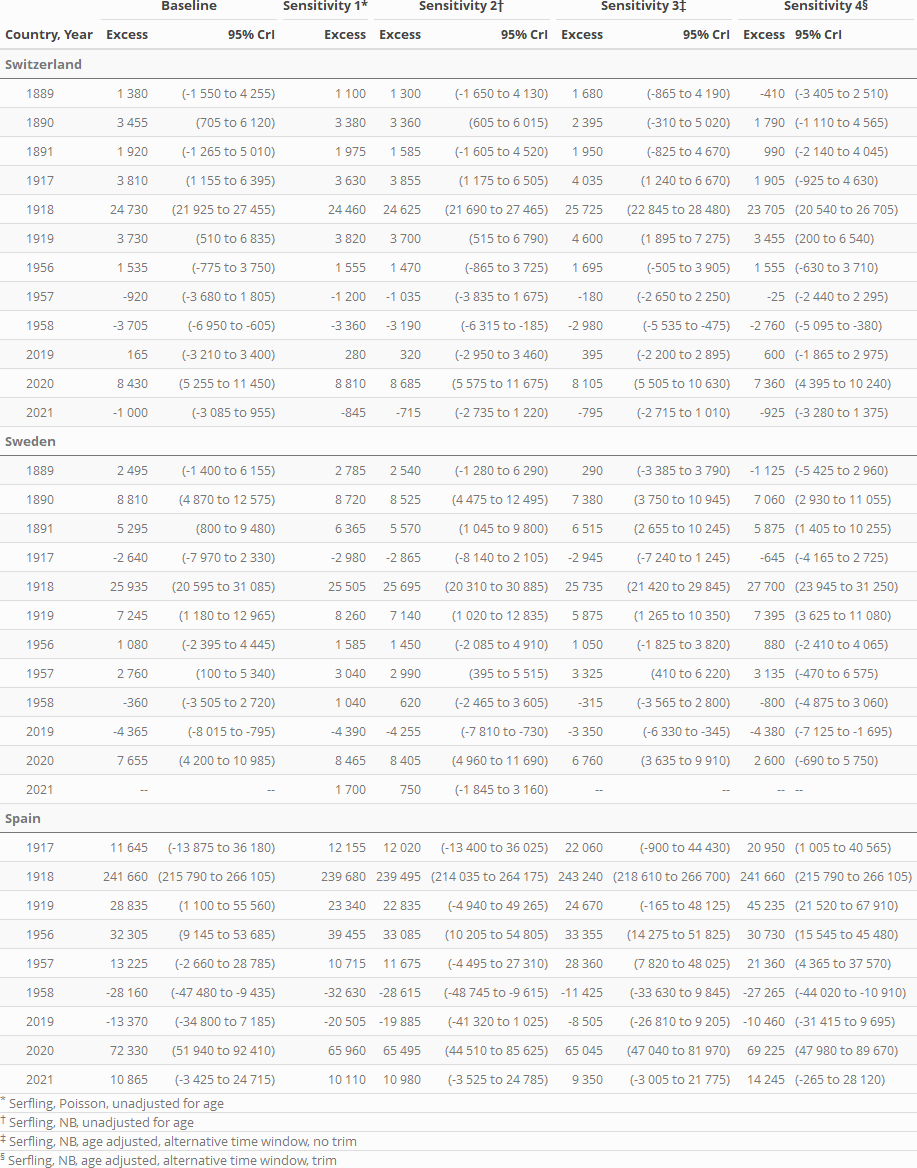
\includegraphics[width=\linewidth]{../Table_S1.png}
	\end{figure}
	
	Table S1: Results of four sensitivity analyses for selected years.  
	
	\section{Supplementary figures}
	
	\begin{figure}[H]
		\centering	
		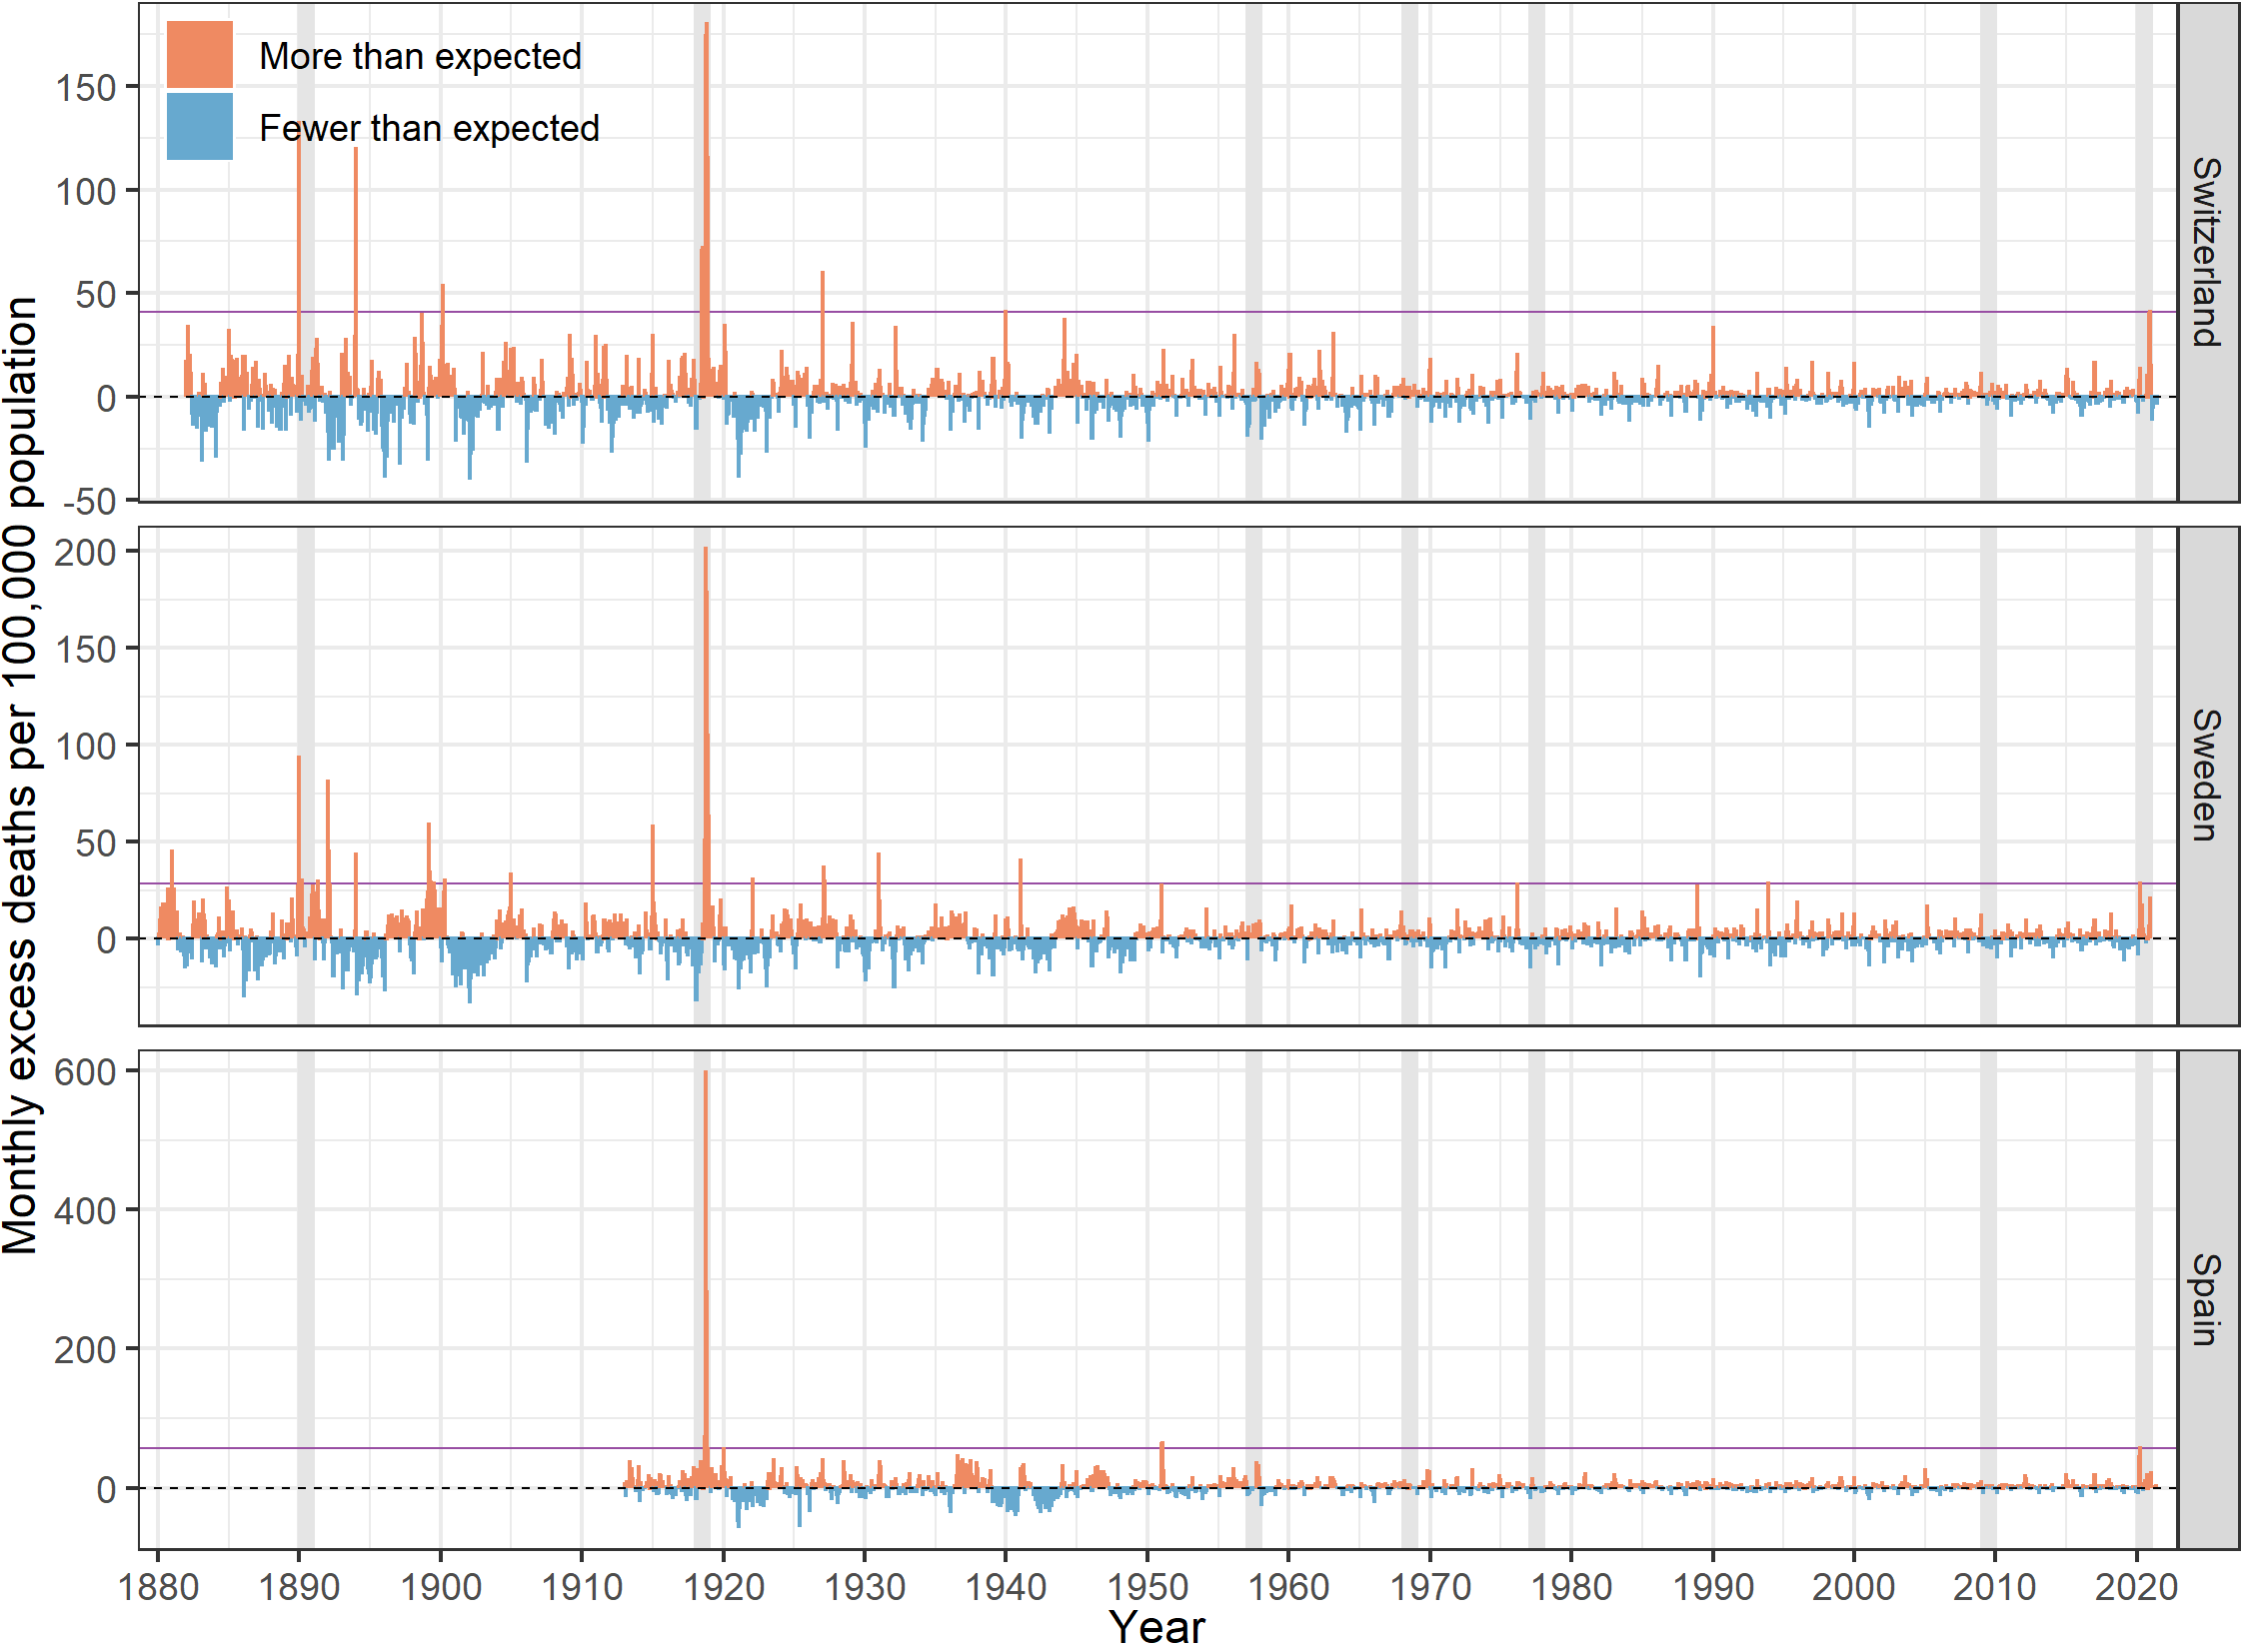
\includegraphics[width=\linewidth]{../Figure_S2b.png}
		\caption{Monthly numbers of deaths in Spain, Sweden, and Switzerland, displayed as differences between observed and expected number of deaths per 100,000 population (red=more, blue=less). The purple horizontal line marks the level of highest value from 20202021 period.}
	\end{figure}

	
	\begin{figure}[H]
		\centering	
		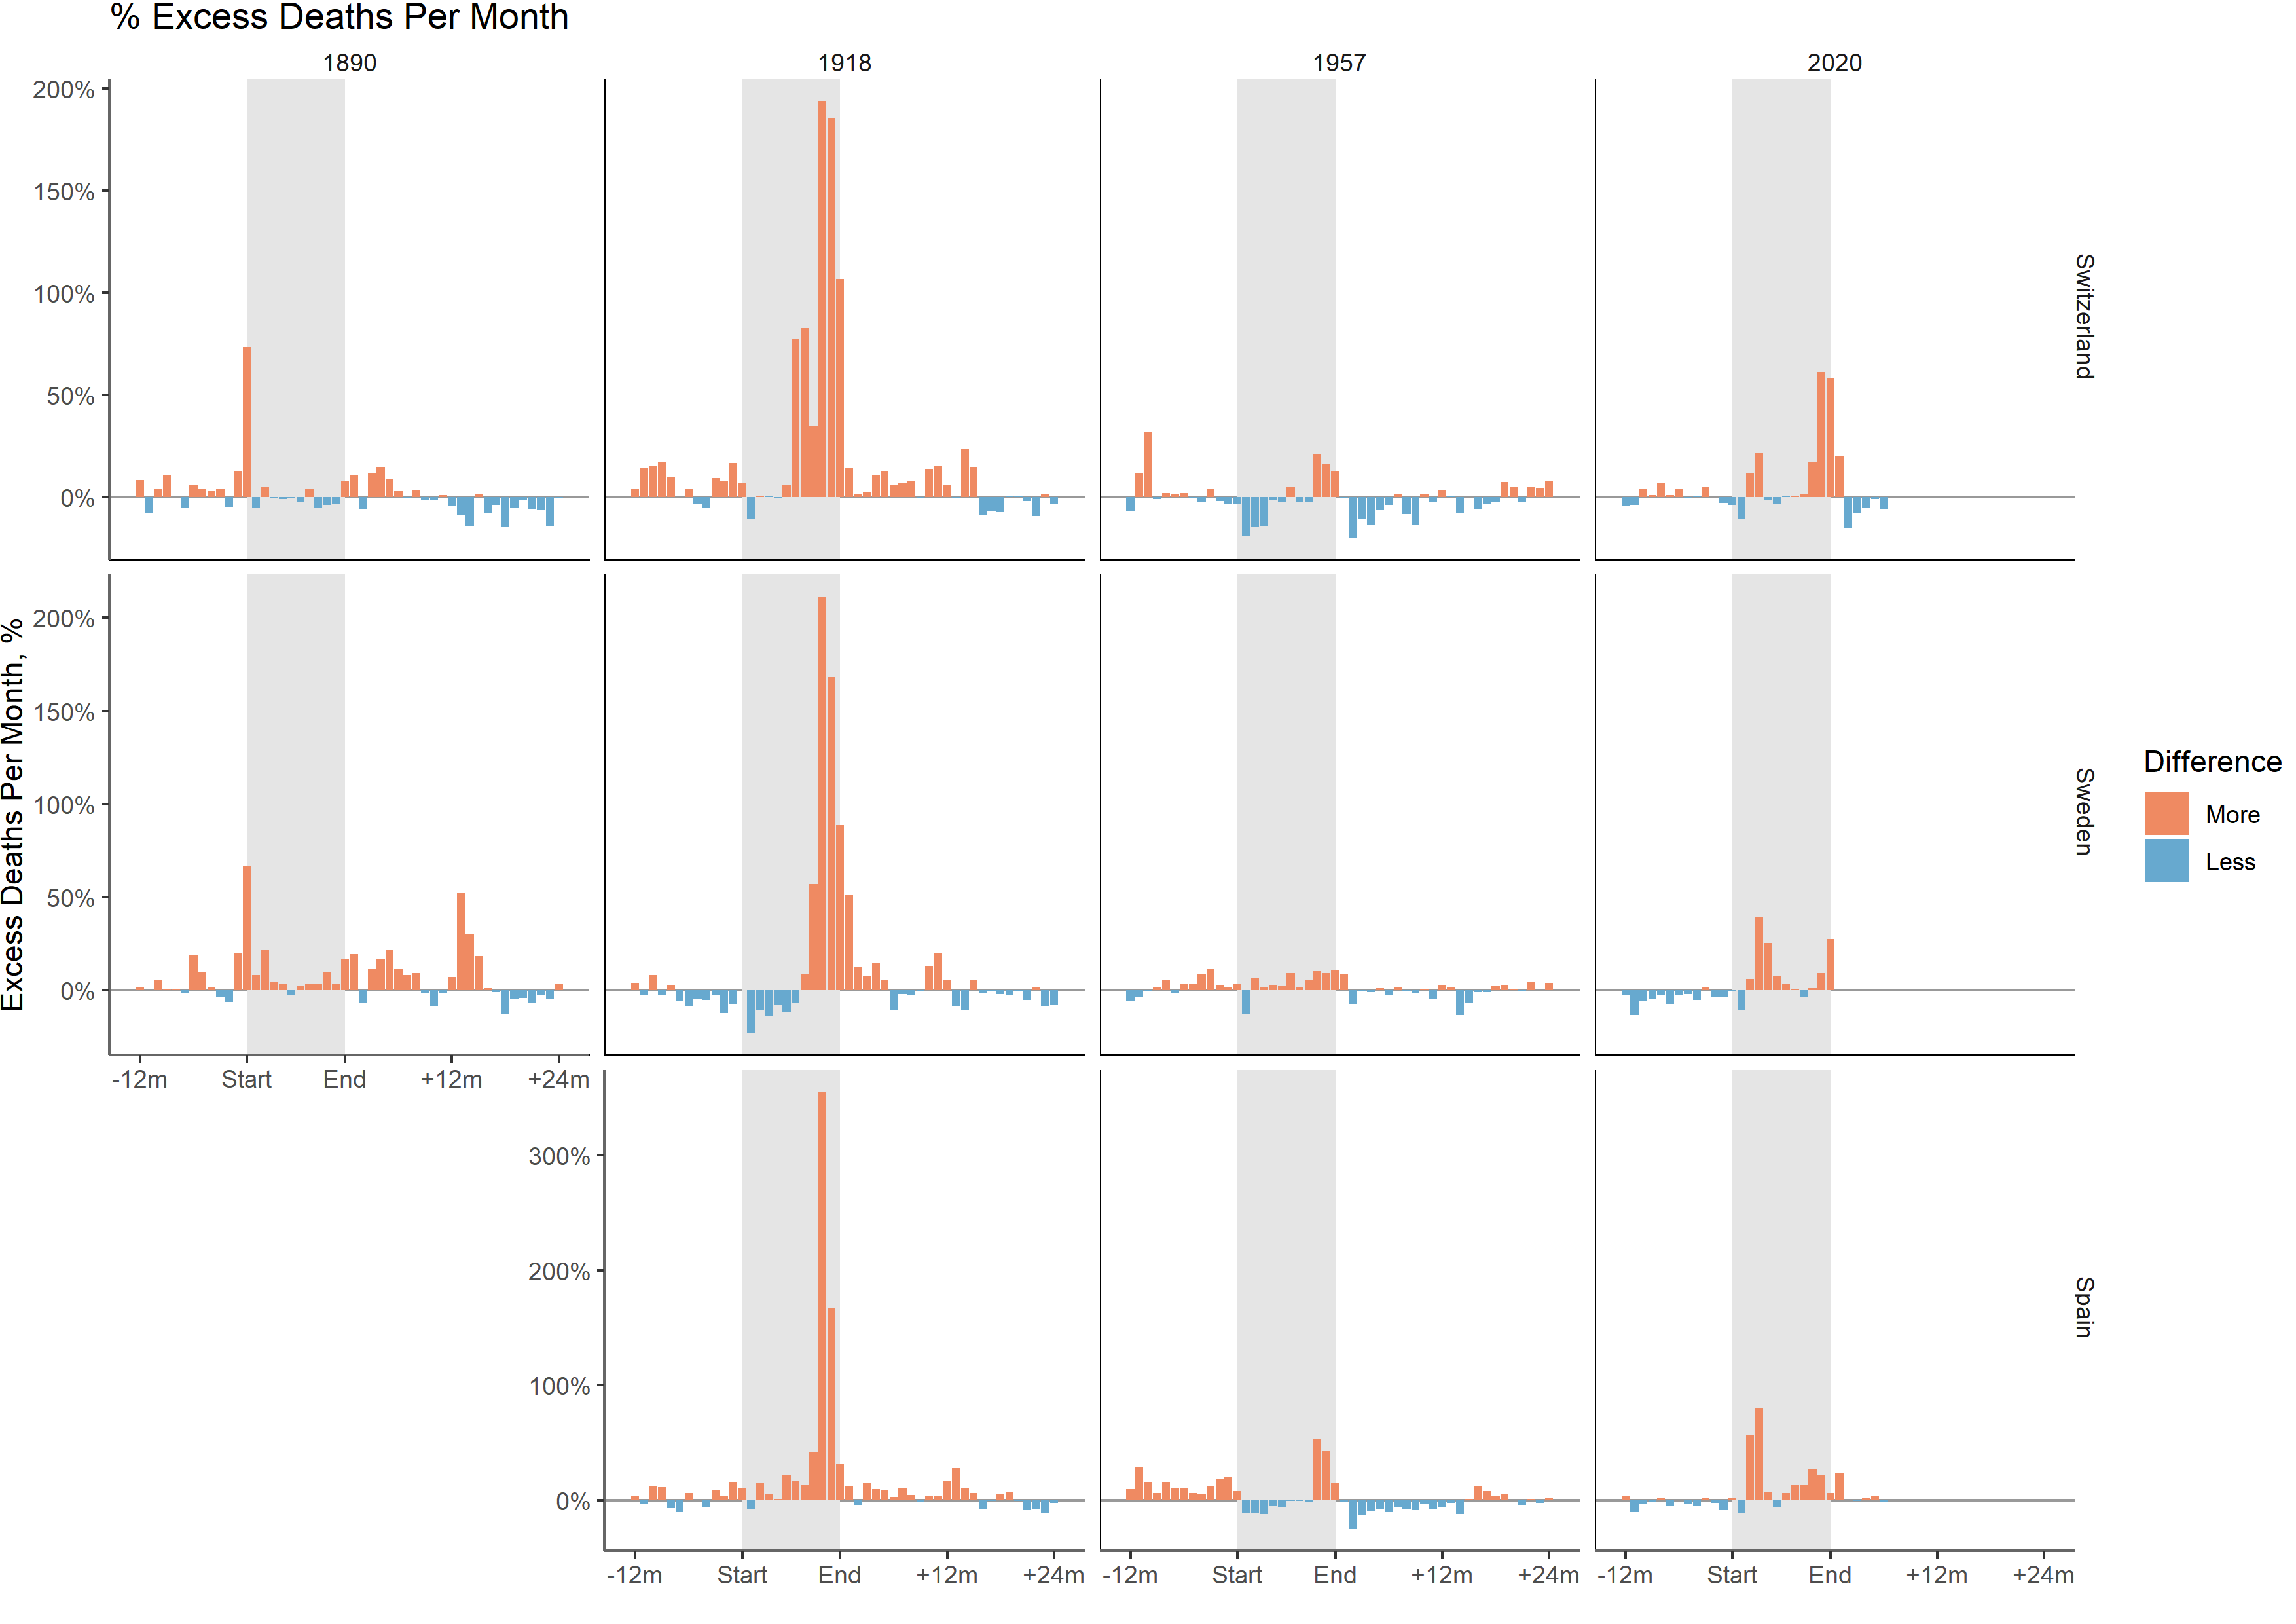
\includegraphics[width=\linewidth]{../Figure_S3b.png}
		\caption{Detailed inspection of the strongest pandemic years 1890, 1918, 1957, and 2020 in all three countries. The differences between observed and expected values (red=more, blue=less) are displayed as percentages.}
	\end{figure}

	
	\begin{figure}[H]
		\centering	
		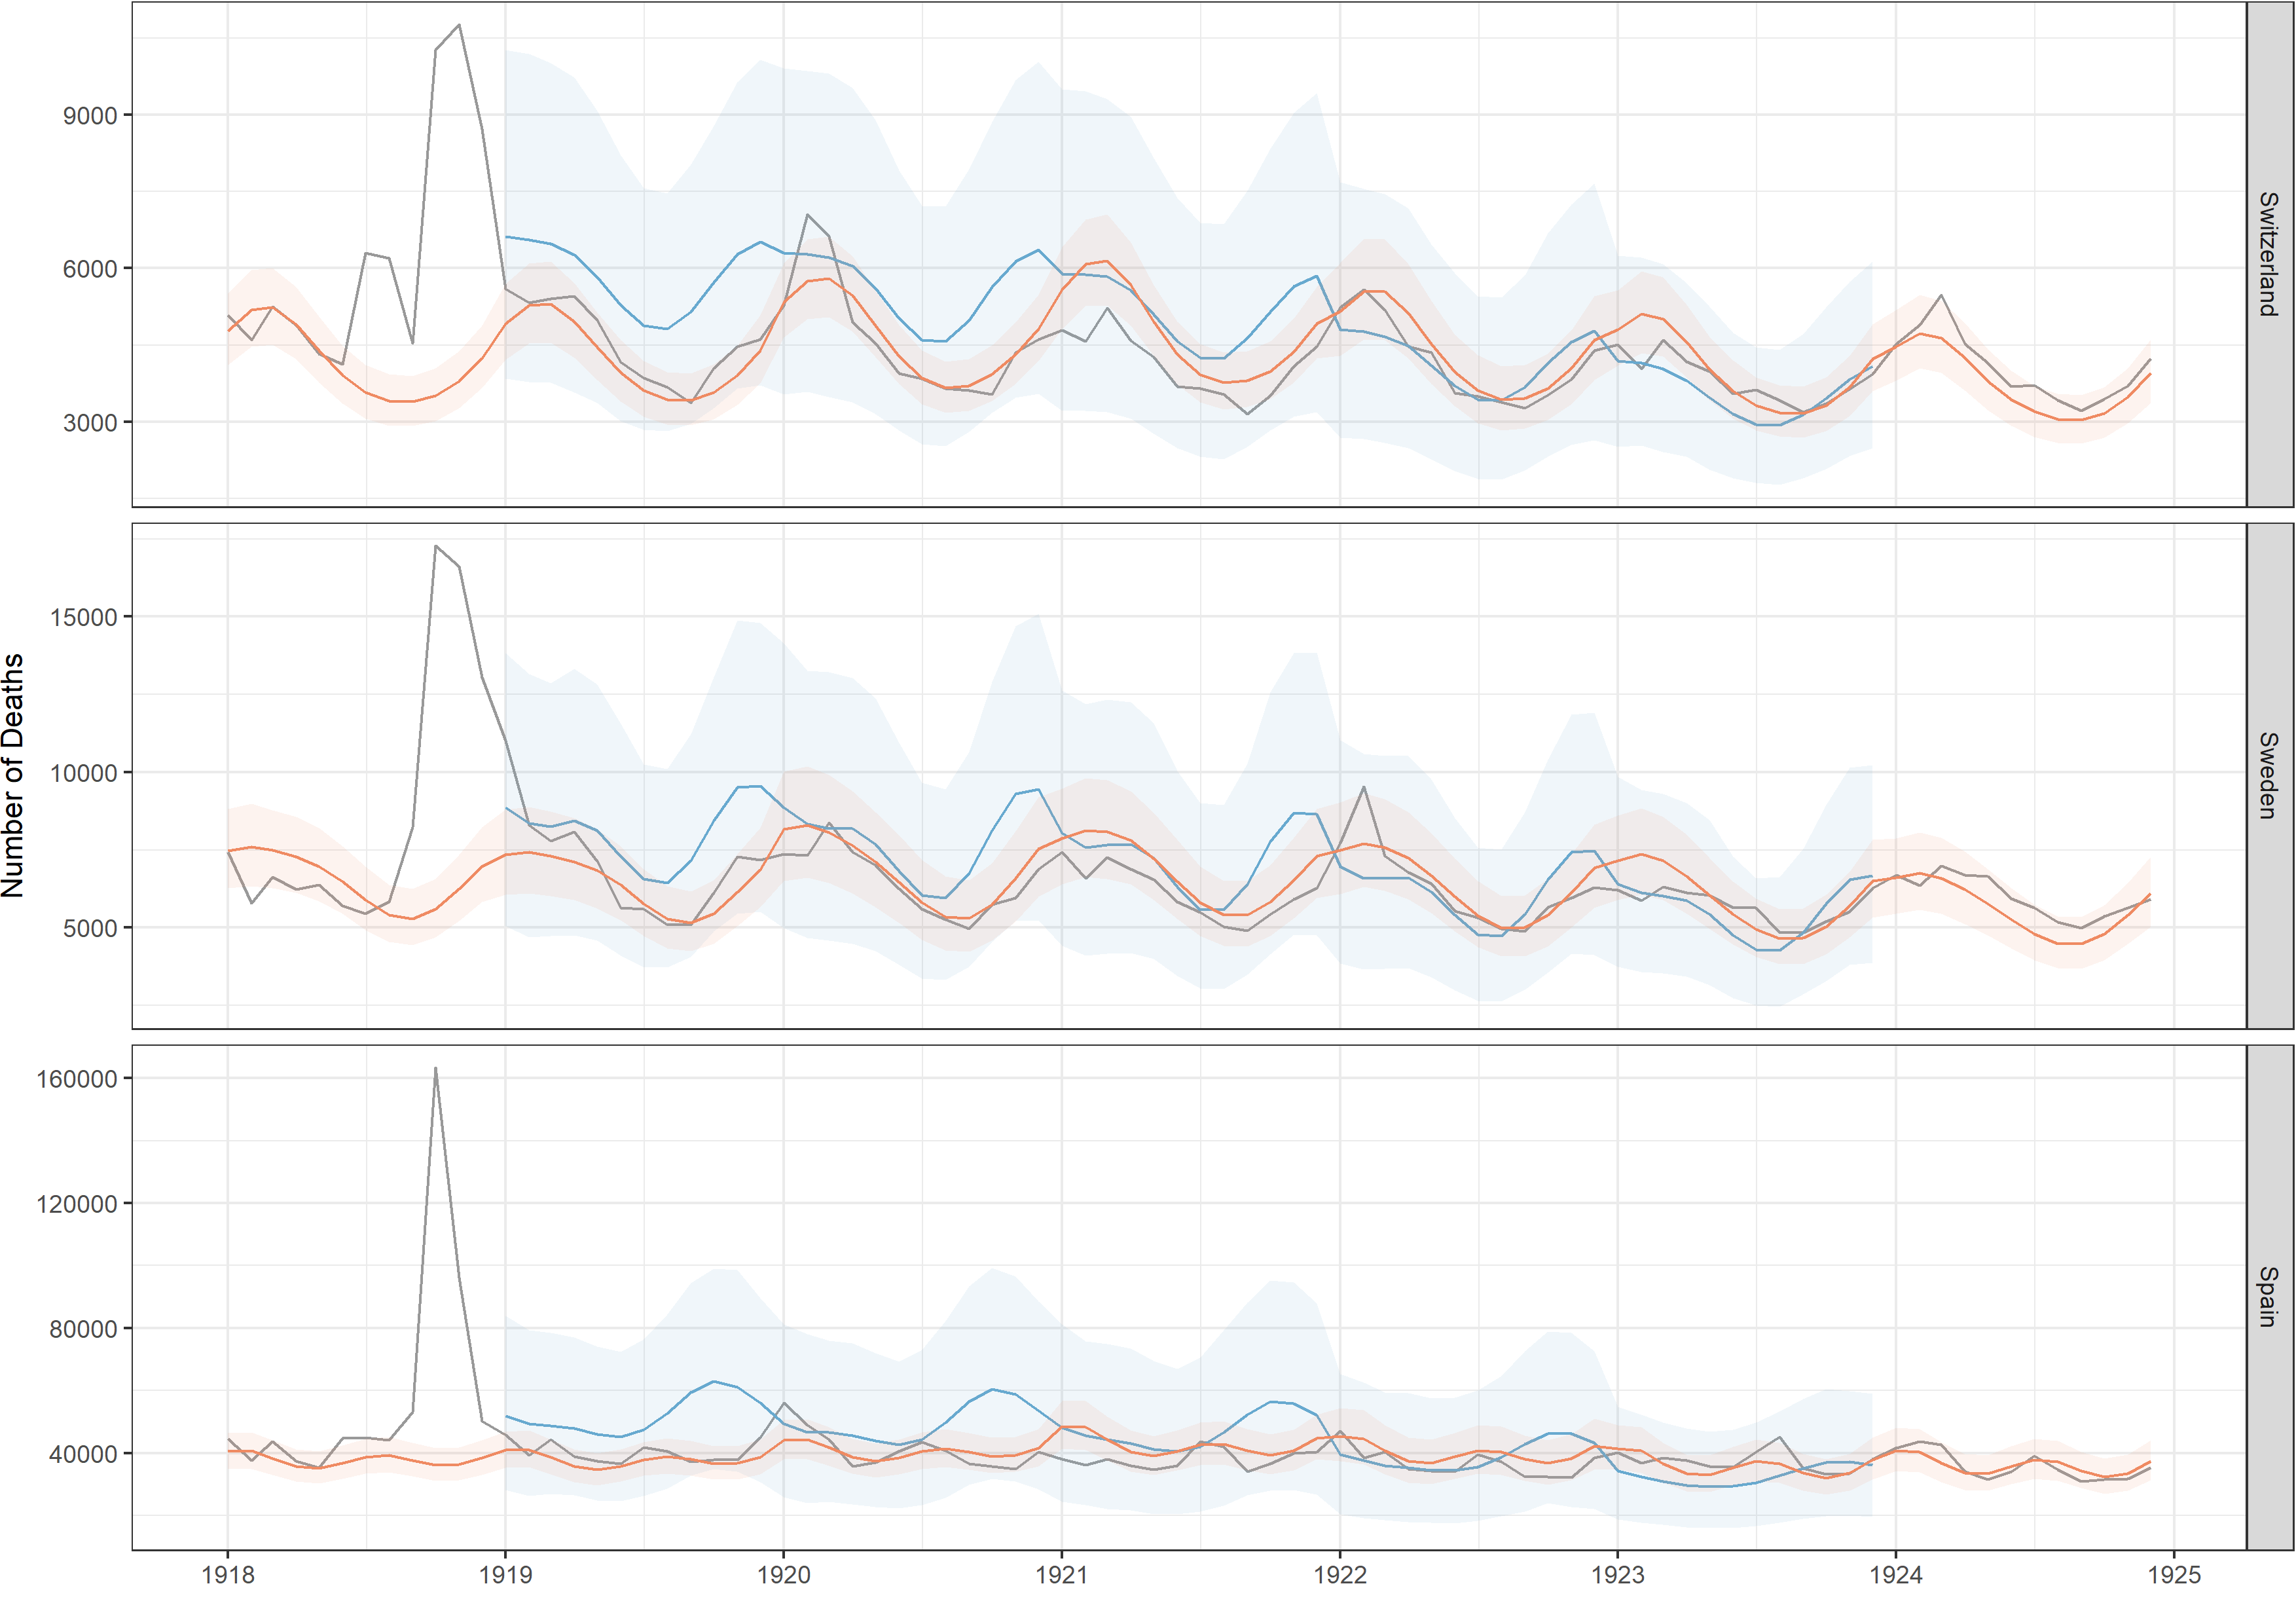
\includegraphics[width=\linewidth]{../Figure_S6a.png}
		\caption{Exemplary visualization based on 1918, how big the difference in the calculated expected number of deaths is for the years 1919 and following, if the year 1918 is included in the calculations (blue line and confidence interval) or not (red line and confidence interval) (Black line: observed deaths). From 1924 onward the results of two methods are the same. }
	\end{figure}
	
	\begin{figure}[H]
		\centering	
		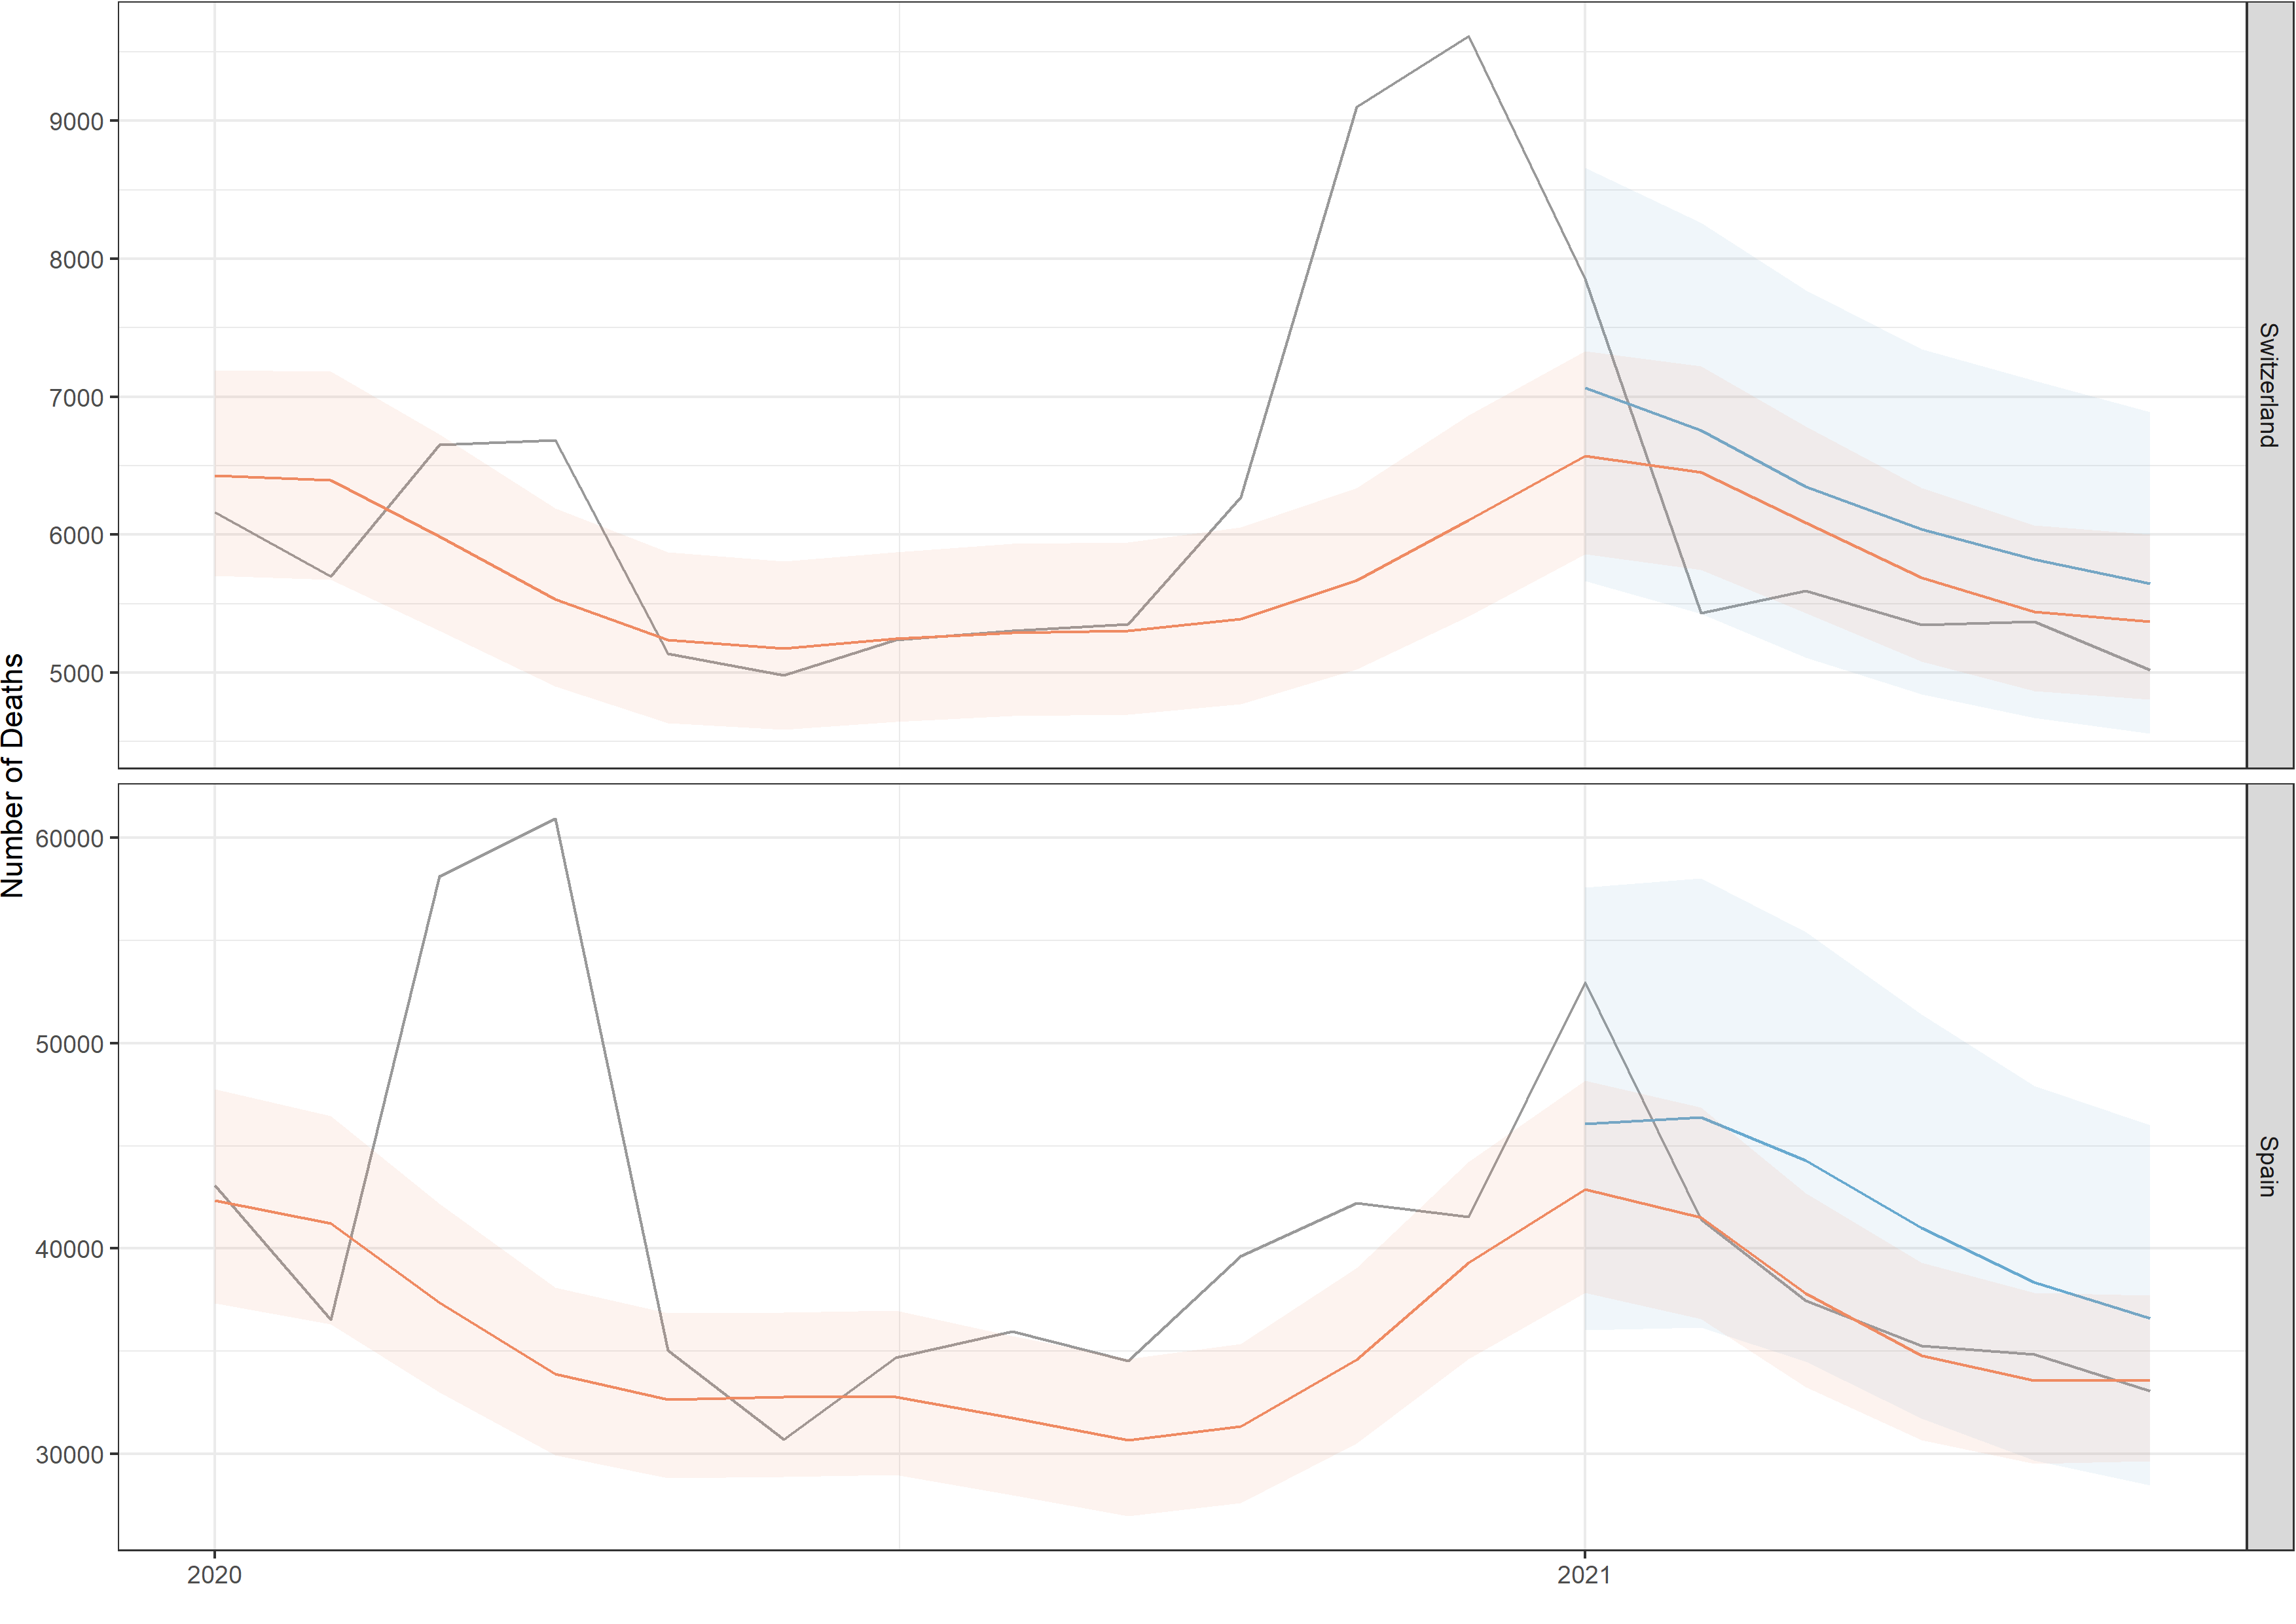
\includegraphics[width=\linewidth]{../Figure_S6b.png}
		\caption{Exemplary visualization based on 2020, how big the difference in the calculated expected number of deaths is for the first six months of the year 2021, if the year 2020 is included in the calculations (blue line and confidence interval) or not (red line and confidence interval) (Black line: observed deaths). }
	\end{figure}



%\section{Supplementary table }

	
	\clearpage


	\bibliography{sup_bib}
	\bibliographystyle{vancouver}
		
	
\end{document}